% 
% Lecture Template for ME3023 -  Measurements in Mechanical Systems - Tennessee Technological University
%
% Spring 2020 - Summer 2020 - Fall 2020
% Tristan Hill, May 07, 2020 - June 12, 2020 - August 23, 2020
% Module 1 - Introduction
% Topic 2 - Types of Variables
% 
%

\documentclass{beamer}                         % for presentation (has nav buttons at bottom)
%\documentclass[handout]{beamer}  % for handout 
\usepackage{beamerthemesplit}
\usepackage{amsmath}
\usepackage{listings}
\usepackage{multicol}
\usepackage{framed}

\beamertemplateballitem 


\definecolor{TTUpurple}{rgb}{0.3098, 0.1607, 0.5176} % TTU Purple (primary)
\definecolor{TTUgold}{rgb}{1.0000, 0.8666, 0.0000} % TTU Gold (primary)

\setbeamercolor{palette primary}{bg=TTUpurple,fg=TTUgold}
\setbeamercolor{palette secondary}{bg=black,fg=TTUgold}
\setbeamercolor{palette tertiary}{bg=black,fg=TTUpurple}
\setbeamercolor{palette quaternary}{bg=TTUgold,fg=black}
\setbeamercolor{structure}{fg=TTUpurple} % itemize, enumerate, etc
\setbeamercolor{section in toc}{fg=TTUpurple} % TOC sections

% custom colors
\definecolor{TTUpurple}{rgb}{0.3098, 0.1607, 0.5176} % TTU Purple (primary)
\definecolor{TTUgold}{rgb}{1.0000, 0.8666, 0.0000} % TTU Gold (primary) 
\definecolor{mygray}{rgb}{.6, .6, .6}
\definecolor{mypurple}{rgb}{0.6,0.1961,0.8}
\definecolor{mybrown}{rgb}{0.5451,0.2706,0.0745}
\definecolor{mygreen}{rgb}{0, .39, 0}
\definecolor{mypink}{rgb}{0.9960, 0, 0.9960}

% color commands
\newcommand{\R}{\color{red}}
\newcommand{\B}{\color{blue}}
\newcommand{\BR}{\color{mybrown}}
\newcommand{\K}{\color{black}}
\newcommand{\G}{\color{mygreen}}
\newcommand{\PR}{\color{mypurple}}
\newcommand{\PN}{\color{mypink}}
\newcommand{\OR}{\color{TTU}}
\newcommand{\GD}{\color{TTUgold}}


\setbeamercolor{palette primary}{bg=TTUpurple,fg=TTUgold}
\setbeamercolor{palette secondary}{bg=black,fg=TTUgold}
\setbeamercolor{palette tertiary}{bg=black,fg=TTUpurple}
\setbeamercolor{palette quaternary}{bg=TTUgold,fg=black}
\setbeamercolor{structure}{fg=TTUpurple} % itemize, enumerate, etc
\setbeamercolor{section in toc}{fg=TTUpurple} % TOC sections

%\usefonttheme{professionalfonts}

\newcommand{\Lagr}{\mathcal{L}} % lagrangian

\newcommand{\hspcu}{\underline{\hspace{20mm}}} % large horizontal space w underline
\newcommand{\vspccc}{\vspace{6mm}\\} % large vertical space
\newcommand{\vspcc}{\vspace{4mm}\\}   % medium vertical space
\newcommand{\vspc}{\vspace{2mm}\\}     % small vertical space

\newcommand{\hspcccc}{\hspace{10mm}} % large horizontal space
\newcommand{\hspccc}{\hspace{6mm}} % large horizontal space
\newcommand{\hspcc}{\hspace{4mm}}   % medium horizontal space
\newcommand{\hspc}{\hspace{2mm}}     % small horizontal space

\newcommand{\eqscl}{0. 9}     % small horizontal space


\author{ME3023 - Measurements in Mechanical Systems} % original formatting from Mike Renfro, September 21, 2004

\newcommand{\MNUM}{1\hspace{2mm}} % Module number
\newcommand{\TNUM}{2\hspace{2mm}} % Topic number 
\newcommand{\moduletitle}{Introduction}
\newcommand{\topictitle}{Types of Variables} 

\newcommand{\sectiontitleI}{Measured Variable}
\newcommand{\sectiontitleII}{Independent and Dependent Variables}
\newcommand{\sectiontitleIII}{Controlled Variables and Parameters}
\newcommand{\sectiontitleIV}{Extraneous Variables }
\newcommand{\sectiontitleV}{Engineering Example }

% custom box
\newsavebox{\mybox}

\title{Module \MNUM - \moduletitle}

\date{Mechanical Engineering\vspc Tennessee Technological University}

\begin{document}

\lstset{language=MATLAB,basicstyle=\ttfamily\small,showstringspaces=false}

\frame{\titlepage \center\begin{framed}\Large \textbf{Topic \TNUM - \topictitle}\end{framed} \vspace{5mm}}

% Section 0: Outline
\frame{

\large \textbf{Topic \TNUM - \topictitle} \vspace{3mm}\\

\begin{itemize}

	\item \sectiontitleI		\vspc % Section I
	\item \sectiontitleII 	\vspc % Section II
	\item \sectiontitleIII 	\vspc %Section III
	\item \sectiontitleIV 	\vspc %Section IV
	\item \sectiontitleV 	\vspc %Section IV

\end{itemize}

}

% Section 1
\section{\sectiontitleI}
\frame{
\frametitle{\sectiontitleI}

\large{``A {\B measurement} is an act of assigning a specific value to a physical variable. That physical variable
is the {\G measured variable}.''} \vspc
{\tiny Text: Theory and Design of Mech. Meas.}

}

% Section 2
\section{\sectiontitleII}
\frame{
\frametitle{Independent and Dependent Variables}

{``If a change in one variable will not affect the value of some other variable, the
two are considered independent of each other. A variable that can be changed independently of other
variables is known as an {\PR independent variable}. A variable that is affected by changes in one or more
other variables is known as a {\BR dependent variable}. Normally, the variable that we measure depends on
the value of the variables that control the process.''} \vspc
{\tiny Text: Theory and Design of Mech. Meas.}

}

% Section 3
\section{\sectiontitleIII}
\frame{
\frametitle{\sectiontitleIII}

{``A variable is {\B controlled} if it can be held at a constant value
or at some prescribed condition during a measurement... ...complete control of a variable is not usually
possible. We use the adjective {\B controlled} to refer to a variable that can be held as prescribed, at
least in a nominal sense... \vspc
...we define a {\G parameter} as a functional grouping of variables. For example, a moment of inertia or a Reynolds number... ...A {\G parameter} that has an effect on the behavior of the measured variable is called a control parameter....''} \vspc
{\tiny Text: Theory and Design of Mech. Meas.}

}

% Section 4
\section{\sectiontitleIV}
\frame{
\frametitle{\sectiontitleIV}

{``Variables that are not or cannot be controlled during measurement but that affect the value of the
variable measured are called {\R extraneous variables}. Their influence can confuse the clear relation
between cause and effect in a measurement... ...The effects due to {\R extraneous variables} can take the form of signals superimposed
onto the measured signal with such forms as {\PR noise} and drift.''} \vspc
{\tiny Text: Theory and Design of Mech. Meas.}

}
% Section 5
\section{\sectiontitleV}
\frame{
\frametitle{\sectiontitleV}


	\textbf{ SHARP I.R. Ranger - Distance Sensor} \vspc
	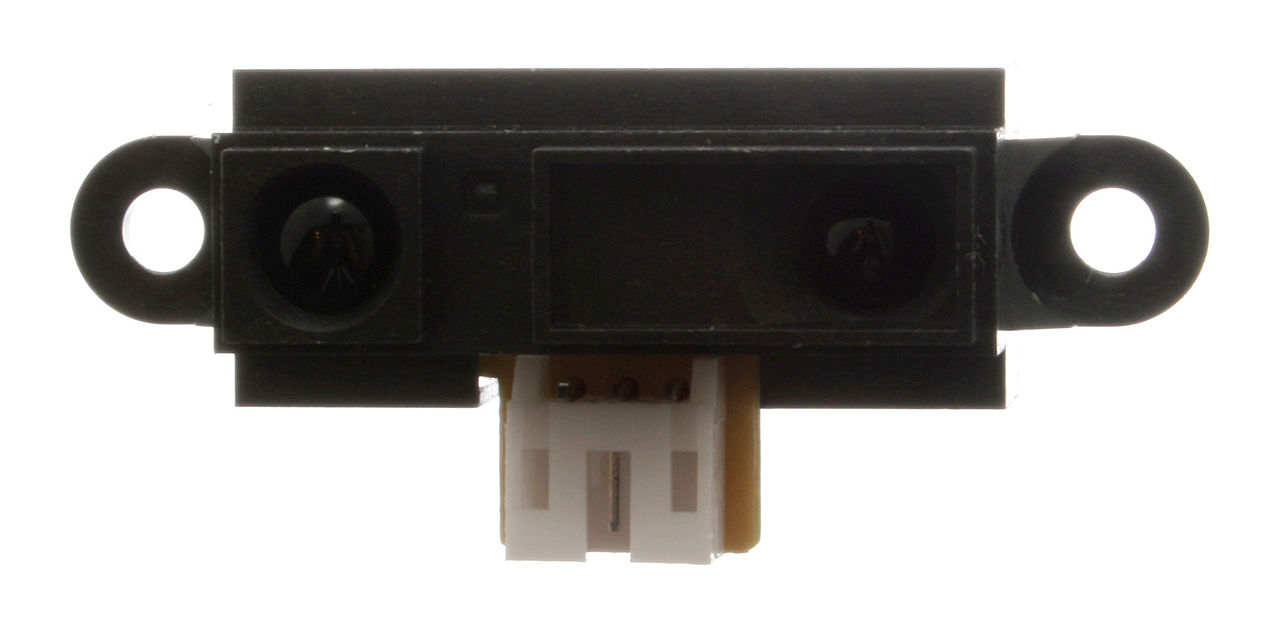
\includegraphics[scale=0.5]{proximity_sensor.jpg} \hspace{20mm}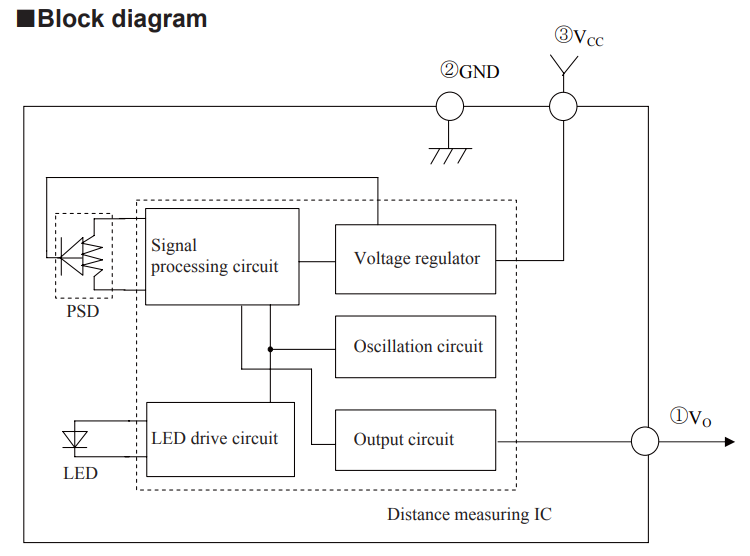
\includegraphics[scale=0.20]{sharp_ranger_circuit.png} \vspc
  {\tiny Image, More Info: \href{https://en.wikipedia.org/wiki/Proximity_sensor}{Wikipedia} }\hspace{40mm} {\tiny Image, More Info: \href{https://en.wikipedia.org/wiki/Position_sensitive_device}{Wikipedia} }

}

\frame{
\frametitle{Engineering Example}


Consider the IR distance ranger, name at least one physical variable for each of the following categories. 

\begin{itemize}
	\item Measured Variable \vspc 
	\item Independent Variable \vspc
	\item Dependent Variables  \vspc 
	\item Controlled Variables  \vspc 
	\item Extraneous Variables  \vspc 
\end{itemize}

}

\end{document}





